
\section{Infrastructure for Verification of Reproducibility}
\label{sec:infrastructure}

The Data Editor manages the infrastructure needed to access data and code, conducts reproducibility checks, and archives and preserves replication packages. In general, the first two infrastructure pieces are provided by the replication team at Cornell University, the latter primarily by the  \aeadcr{} provided by openICPSR at the University of Michigan, with additional support from the AEA's in-house IT staff. In 2022, the Data Editor continued to explore the use of several other infrastructures for  conducting reproducibility checks and for the preservation of data for replication packages.


\subsection{Pre-publication verification of computational reproducibility}
\label{sec:verification}

\paragraph{The process}

Pre-publicaton verification is conducted by the Data Editor's team at Cornell University. 
Requests for assessment of reproducibility are received and assigned to a team member, who then assesses data availability and compliance with requirements. When some data are available, a full or limited reproducibility check is conducted. If we cannot obtain access to the data or computational resources in a timely fashion, we may reach out to third-parties who can, and request a reproducibility check from them. Once all computations have been completed, a process that can take anywhere from a few minutes to several weeks, a report is compiled, reviewed and approved by the Data Editor, and submitted back to journal editors, who handle most communications with the authors. The report will have  one of four possible recommendations (see Table~\ref{tab:responses}). A ``conditional acceptance'' implies that a revision will need to be resubmitted to the Data Editor to address any identified shortcomings. An ``acceptance'' means that no further changes are necessary, and both the manuscript (after copy-editing) and the replication package can be scheduled for publication.%
%
\footnote{Manuscript and replication package are generally published at the same time, though at the request of either editors or authors, the replication package can be published at any time after acceptance.} 
%
However, to streamline processing, we may also recommend an ``acceptance with modifications requested.'' In such cases, the remaining modifications are minor, and can be handled during copy-editing (for instance, a small number of tables need minimal changes) and prior to publication of the replication package (for instance, a fixable error in a program, or a clarification in the README, not affecting any important tables or figures). 


%\begin{table}[t]
\begin{center}
	\captionof{table}{Recommendations}{}
	\label{tab:responses}
	\centering
	
% Table created by stargazer v.5.2 by Marek Hlavac, Harvard University. E-mail: hlavac at fas.harvard.edu
% Date and time: Thu, Mar 02, 2023 - 03:41:54 AM
\begin{tabular}{@{\extracolsep{5pt}} lr} 
\toprule 
Response option & Frequency \\ 
\midrule Accept & 48 \\ 
Accept - with Changes & 231 \\ 
Conditional Accept & 32 \\ 
Revise and Resubmit & 5 \\ 
\bottomrule 
\end{tabular} 

 \end{center}
%\end{table}

We have increasingly made use of this feature. While we check that authors comply with the request for modifications, no further computational assessment is made. A recommendation of  ``revise and resubmit'' is recorded when we receive a request prior to a conditional acceptance, i.e., during the ``R\&R'' phase. When we have serious concerns, we will reach out directly to the responsible editor, and discuss solutions with the authors. 

\paragraph{Assessments made}

Between \firstday{} and \lastday{}, the AEA Data Editor team  received
\jiraissues{} requests,  for \jiramcs{} manuscripts.%
%
\footnote{This includes only requests submitted between those dates, and does not take into account in-progress requests on \firstday{}.}
%
Requests typically are channeled to the team by the AEA's journal submission and review system, but others were initiated by authors or editors directly, often while preparing the replication materials. Of these,  \jiraissuescplt{} reports (\jiramcscplt{} manuscripts) were submitted back to editors,\footnote{The balance are either in progress or are not coded in the adminstrative system as having been submitted to ScholarOne, such as replication packages for Papers and Proceedings.} and \jiramcspending{} were completed up to the point of publication of the data deposit, including any post-acceptance modifications.  Table~\ref{tab:responses} shows the distribution of the last recommendation on record for manuscripts as of \lastday{}.  Table~\ref{tab:jirastats} breaks these numbers down by journal, showing the number of requests received (``rcvd'') and  reports completed (``cplt'') in the left panel. The right panel shows the number of manuscripts for which one or more requests were received (``rcvd'') and reports completed (``cplt''). The columns marked ``ext.'' identify cases where we reached out to external replicators, which we discuss later. Finally, the last column identifies manuscripts for which the entire process has been completed, and which are ``pending'' publication.
%

\begin{table}[]
    \caption{Processing Statistics}
    \label{tab:jirastats}
    \small
    \begin{threeparttable}
    \centering
    
% Table created by stargazer v.5.2 by Marek Hlavac, Harvard University. E-mail: hlavac at fas.harvard.edu
% Date and time: Thu, Dec 08, 2022 - 04:38:18 PM
\begin{tabular}{@{\extracolsep{5pt}} lrrrrrrr} 
\toprule 
        & \multicolumn{3}{c}{Issues} & \multicolumn{4}{c}{Manuscripts}\\
        \cmidrule{2-4}\cmidrule{5-8}
Journal &  (rcvd) &  (cplt) &  (ext.) &  (rcvd) &  (cplt) &  (ext.) &  (pend.) \\ 
\midrule 
AEJ:Applied Economics & 112 & 91 & --- & 72 & 67 & --- & 29 \\ 
AEJ:Economic Policy & 57 & 48 & 2 & 54 & 45 & 2 & 25 \\ 
AEJ:Macro & 52 & 45 & 4 & 45 & 41 & 4 & 21 \\ 
AEJ:Micro & 20 & 18 & 1 & 18 & 16 & 1 & 6 \\ 
AER & 103 & 83 & 1 & 96 & 78 & 1 & 64 \\ 
AER:Insights & 33 & 28 & 1 & 30 & 26 & 1 & 19 \\ 
JEL & 26 & 22 & --- & 21 & 19 & --- & 15 \\ 
JEP & 27 & 26 & 1 & 24 & 24 & 1 & 21 \\ 
Totals & 500 & 361 & 10 & 429 & 316 & 10 & 257 \\ 
\bottomrule 
\end{tabular} 

    \begin{tablenotes}
    \item[] \textit{Notes:} Data for requests received by the AEA Data Editor between \firstday{} and \lastday{}. AEA P\&P are excluded from this table. See text for details.
    \end{tablenotes}
 \end{threeparttable}
   \end{table}





\paragraph{Issues encountered}


\subparagraph{Incomplete data provenance and data availability:} Most articles still provide imprecise or incorrect information regarding access to data that is not provided. In some cases, authors fail to provide data that should be provided, and in other cases, authors inadvertently provide data for which they do not have redistribution rights. Our impression is that there is improvement over the year, but we do not formally capture this as part of our reporting.

\subparagraph{Specification of computational environment:}
Sufficiently precise descriptions of the required auxiliary packages or libraries, as ``manifest''-like files in R, Python, and Julia, or as "\texttt{setup.do}"-like programs in Stata remain rare. This has not changed much either, and there remains much room for improvement. We have seen only a handful of packages use containers (``Docker''), and we have used containers in a few additional verifications. We continue to work with some users to leverage such environments (see our discussion later under \textit{Computational Infrastructure}).

\subparagraph{Incomplete instructions and manual manipulation:} Heuristically, the number of manual instructions to run code, or to save tables and figures, which detract from speedy and efficient reproduction by third parties, remain too high. 


\paragraph{Delays} 

A recurring concern expressed by authors, editors, and staff members are delays in publication, due to the verification process. The median manuscript is reviewed once (Table~\ref{tab:pre:rounds} shows the breakout by journal).
%
We have continued to reduce the number of rounds before a paper is accepted by accepting replication packages subject to minor post-acceptance edits (the ``accept with changes'' decision described earlier). Figure~\ref{fig:rounds} illustrates the difference graphically, by journal. This comes with additional challenges, since authors are less responsive for subsequent (but still necessary) change requests prior to publication. 

Additional delays were encountered this year due to training and hiring challenges. We train three times a year for acceptance in the LDI Lab, and continue to have an excellent retention rate of lab members once trained. However, at each of this year's training events, students have been unable to attend at the last minute. Failure to attend the intensive one-day training is highly correlated with later retention and efficiency. We are addressing these issues through increased recruiting for the training, and expansion of the pool of participants.



\begin{table}
    \centering
    \caption{Assessment rounds for completed manuscripts}
    \label{tab:pre:rounds}
    \begin{threeparttable}
    \centering
    
% Table created by stargazer v.5.2 by Marek Hlavac, Harvard University. E-mail: hlavac at fas.harvard.edu
% Date and time: Thu, Mar 02, 2023 - 03:41:56 AM
\begin{tabular}{@{\extracolsep{5pt}} ccccccc} 
\toprule 
Rounds & AER & AER Insights & AEJ Applied & AEJ Macro & AEJ Micro & AEJ Policy \\ 
\midrule 1 & 64 & 20 & 37 & 32 & 12 & 38 \\ 
2 & 7 & 2 & 3 & 3 & 0 & 3 \\ 
\bottomrule 
\end{tabular} 

    \begin{tablenotes}
    \footnotesize
    \item[] \textit{Notes:} Data for papers first sent to the AEA Data Editor between \firstday{} and \lastday{}, and for which all rounds have been completed. AEA P\&P, JEP, and JEL are excluded from this table. See text for details. Numbers differ slightly between this table and Table~\ref{tab:jirastats} because they are extracted from two different administrative systems, with different timing cutoffs.
    \end{tablenotes}
 \end{threeparttable}
\end{table}

\begin{figure}
    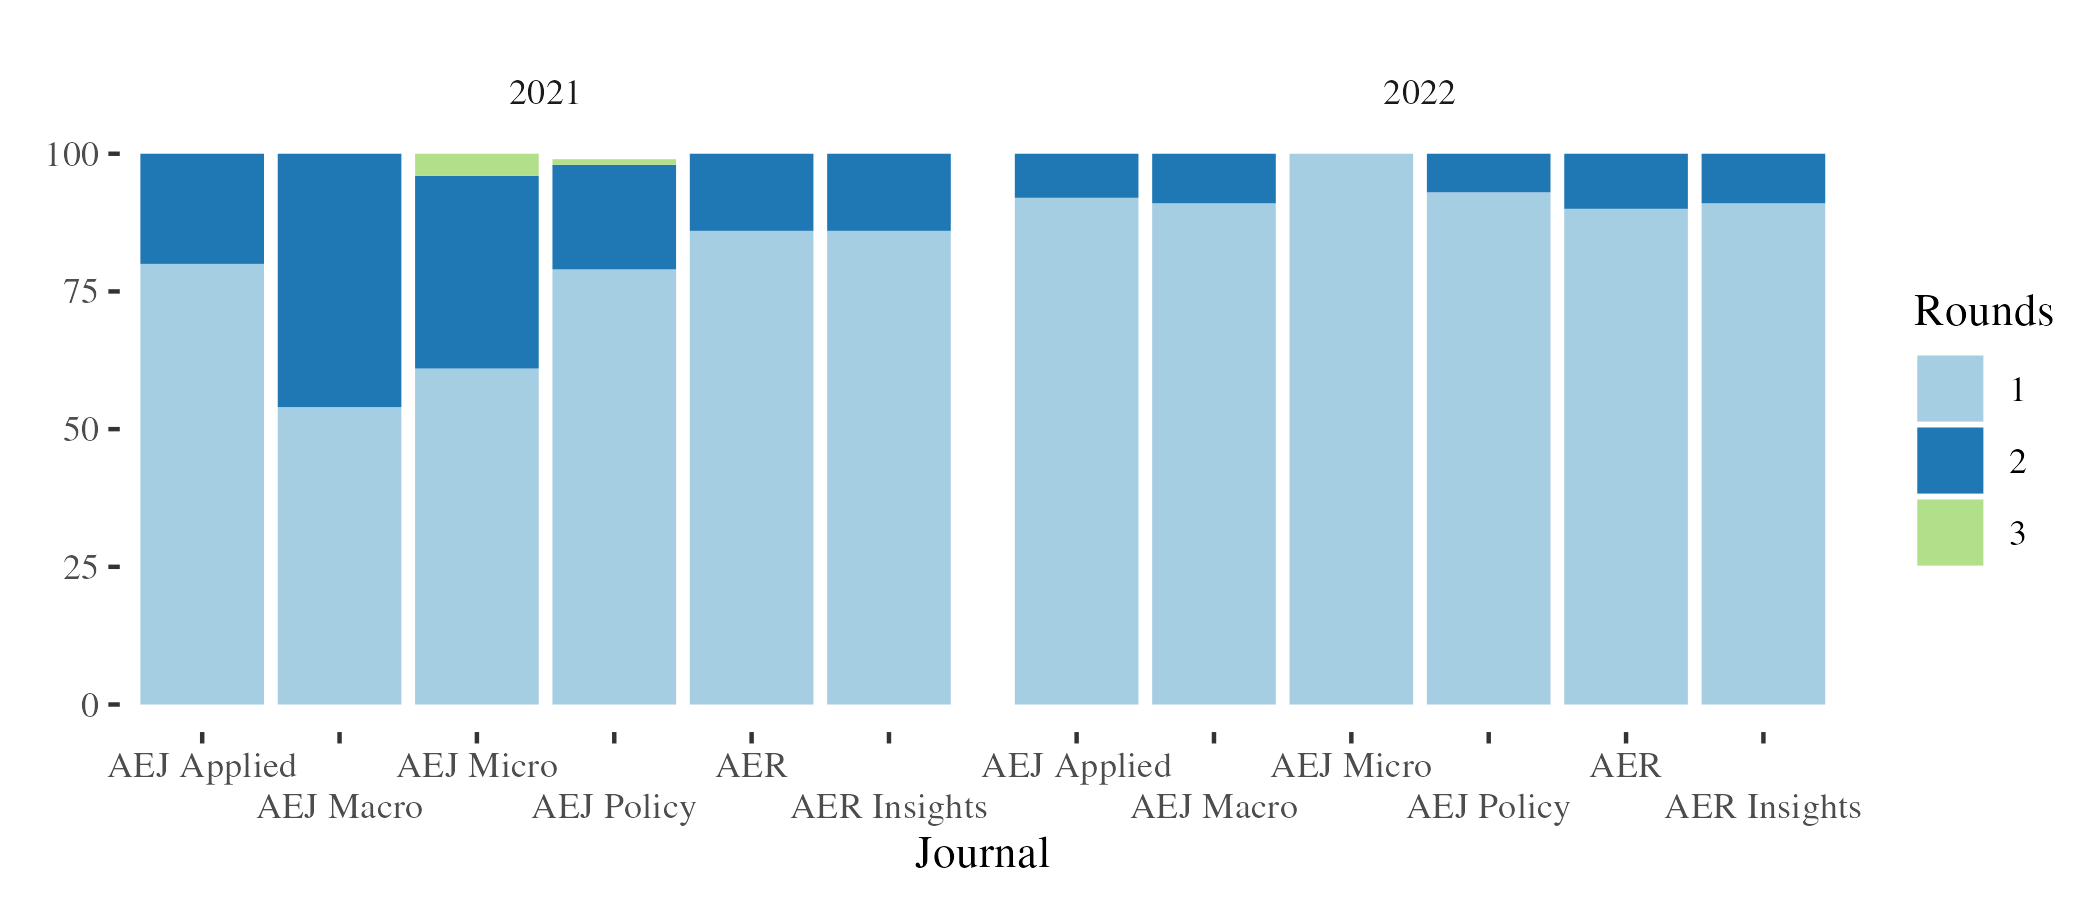
\includegraphics[width=\textwidth]{images/plot_rounds_compare.png}
    \centering
    \caption{Comparing rounds per journal between 2021 and 2022\label{fig:rounds}}
\end{figure}

\paragraph{Disseminating process information}

We continue to improve our documentation, based on careful monitoring of the process, and where more information could be beneficial. Our documentation aims to (a) provide authors with the information as early as possible, when it is still easy to include reproducible practices in projects at relatively low cost and (b) provide authors with the best information, to reduce frictions and uncertainty. Authors are provided with an informational form upon submission, and a short form, provided upon conditional acceptance, collects salient information about the replication package, but also links to important guidance.%
\footnote{These forms can also be found at \href{https://www.aeaweb.org/journals/data}{aeaweb.org/journals/data}.} 
We now require that authors provide the information as per the Social Science Data Editors' template ``README'' \citep{READMEv1.1.0}, an improved version of which  was introduced in November 2022 after feedback from authors and consultation amongst multiple data editors (see Section~\ref{sec:infrastructure}). 

\paragraph{Computational Infrastructure}

Most replication packages are computationally verified by replicators on the computers available to the Data Editor at the Cornell University Economics Department and the ILR School. The majority are handled on the Windows Server systems of the Cornell Center for Social Sciences, while some are run on the Linux-based Bioinformatics cluster. Occasionally, personal macOS laptops are used. Systems can handle memory requirements up to 1024 GB or up to 100 cores. 

While these systems are fairly standard, they cannot cover all scenarios described in authors' computational requirements. Furthermore, these systems, much like the authors' own systems, are not shareable more broadly, and thus sometimes make it difficult to control for specific requirements, or to share error messages in the most reproducible way.  

We continue to leverage additional computational environments. We have used \curlcite{https://codeocean.com}{CodeOcean} \citep{clyburne-sherin_computational_2019} both to share active (but only partially successful) reproduction efforts and to publish reproducible ``capsules.'' We collaborate with the team behind ``WholeTale'' \citep{BrinckmanFutureGener.Comput.Syst.2018} and the Odum Institute, which conducts reproducibility checks for various political science journals. Both {{CodeOcean}} and WholeTale rely on containerization, often known under the commercial name ``Docker,'' which can be independently used to precisely define and then share computational environments. We use containers through CodeOcean and or WholeTale, when appropriate. We use Docker on the Linux cluster at Cornell University, or on Linux workstations or macOS laptops amongst the LDI lab members when storage or compute resources are insufficient at the public providers. Sample code  can be found at the \purlcite{https://github.com/AEADataEditor/}{AEA Data Editor's Github repository}. Pre-configured Stata and manuscript-specific Docker images can be found at Docker Hub.\footnote{Generic images are at \href{https://hub.docker.com/u/dataeditors}{hub.docker.com/u/dataeditors}, specific images at \href{https://hub.docker.com/u/aeadataeditor}{hub.docker.com/u/aeadataeditor}.} A more expansive overview of containerization issues in economics can be found at \citet{aea_data_editor_use_2021}.


\subsection{Archive for Replication Packages}


\begin{table}[t]
    \centering
    \caption{Deposit statistics}
    \label{tab:webstats}
     \begin{threeparttable}
     
% Table created by stargazer v.5.2 by Marek Hlavac, Harvard University. E-mail: hlavac at fas.harvard.edu
% Date and time: Thu, Mar 02, 2023 - 03:42:01 AM
\begin{tabular}{@{\extracolsep{5pt}} ccccccc} 
\toprule 
Repository & Published & Downloads & Views & Uploads & Files & Size (GB) \\ 
\midrule ICPSR & 4,171 & 297,660 & 2,527,869 & 427 & 51,394 & 951.48 \\ 
Zenodo & 9 & 284 & 633 & 4 & 6,163 & 372.6 \\ 
\bottomrule 
\end{tabular} 

 
    \begin{tablenotes}
    \footnotesize
    \item[] \textit{Note}: Unit of observation are deposits at the named repository. Columns 1-3 are for all currently published deposits as of \pkglastday{}. Columns 4-6 are for deposits made between \firstday{} and \pkglastday{}. The number of uploads may not correspond to the number of manuscripts processed by the Data Editor team. Not all uploads have been published yet. 
    \end{tablenotes}
    \end{threeparttable}
\end{table}


The default archive for replication packages accompanying articles in AEA journals is the \aeadcr{}. Deposit instructions are provided on the Data Editor's website, and mentioned upon conditional acceptance. However, it is not the only acceptable archive, as we discuss below.


Table~\ref{tab:webstats} shows statistics for all currently published replication packages at the \aeadcr{}.  There are currently  
\icpsrtotalPublished{} published replication packages.  Between \firstday{} and \pkglastday{}, \pkgcount{} deposits were made, with over \pkgfilesT{} thousand files and nearly 1 TB of data. 

In the past year, the median package size was  \pkgsizemedian{} MB, but a significant number of packages (\pkgsizetwog{} percent) had  packages larger than 2GB. \pkgsizetwentyg{} percent of deposits were larger than 20GB. Note that any partial data packages over 30 GB, the default quota for a deposit, are archived elsewhere. One possible repository is Zenodo, where the  ``AEA Zenodo community'' is available. Table~\ref{tab:webstats} shows a small number of very large packages, with \zenodototalSizeGB{}~GB of data already deposited in only \zenodototalPublished{} packages. 

Some packages have more than 1,000 files, hitting a technical constraint on openICPSR. Provision of opaque ZIP files are generally prohibited. Instructions on how to proceed when file numbers are large, while maintaining maximum visibility onto the file and package structure, are provided on the website. Authors with large packages, or packages with more than 1,000 files, should contact the AEA Data Editor. Depositing at other trusted repositories is one option, described in the next section.

Since the migration to the \aeadcr{}, these replication packages have been viewed \icpsrtotalViewsM{} million times and downloaded nearly \icpsrtotalDownloadsHT{} hundred thousand times.




%\subsection{Migrating Historical Supplements}
%\label{sec:migration}
%
%We  migrated the bulk of historical data (and code) supplements in 2019, from ZIP files stored on AEA servers to the \aeadcr{}. A few dozen replication packages are still awaiting migration. Most of these packages either have a very large number of files that surpass technical limitations of the \aeadcr{}, or turned out to be corrupted or illegible in their original version. We are still working on migrating these as resources permit. 
%
%% report on UMich metadata project
%% data provided by email
%
%We reported last year on a project with a research team at the University of Michigan, which solicited metadata improvements to migrated replication packages.  911 researchers provided additional metadata for 522 studies, which were incorporated into the \aeadcr{} in October 2021. We are currently assessing the impact of the improved metadata on findability of such packages.



\begin{figure}[t]
    \centering
    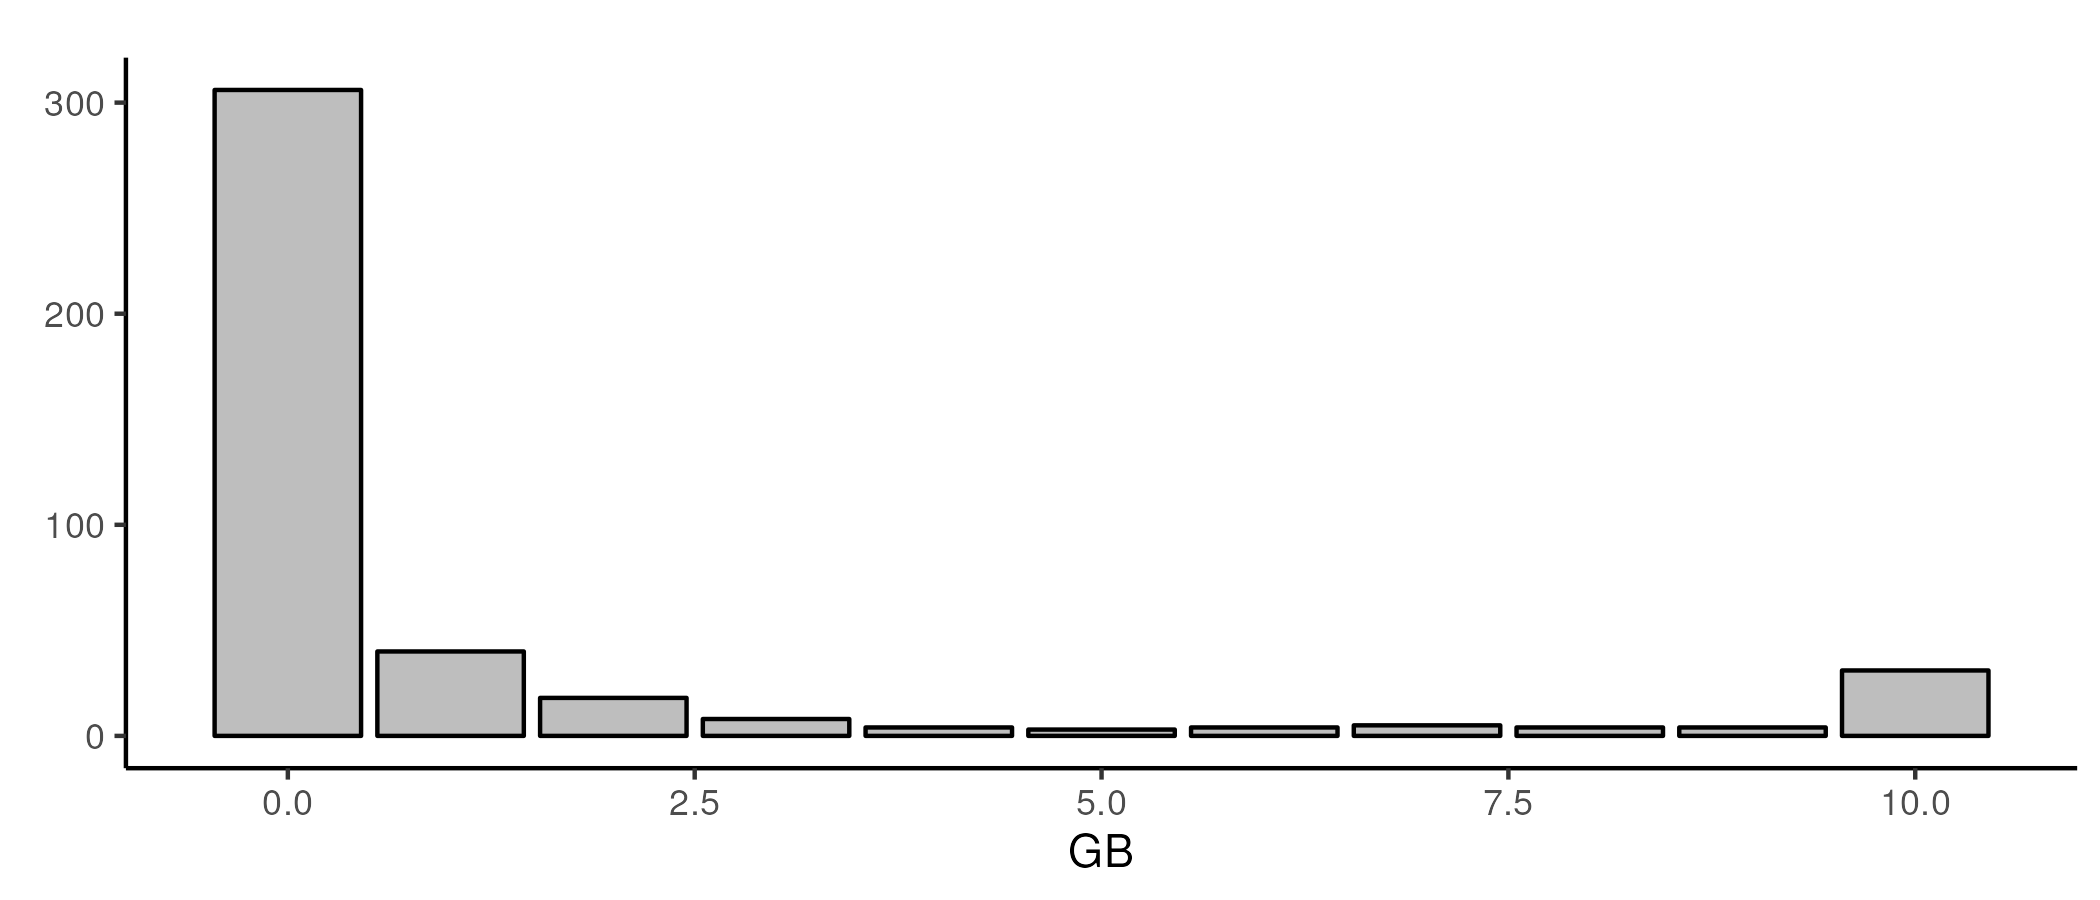
\includegraphics[width=\textwidth]{images/plot_filesize_dist.png} 
    \caption{Size distribution of replication packages deposited at openICPSR between  \firstday{} to \lastday{}, top-coded at 10GB.}
    \label{fig:size_packages}
\end{figure}


\subsection{Third-party repositories}

The \ac{DCAP} allows for code and data  to be deposited at other trusted repositories, as long as all other elements of the \ac{DCAP} are complied with. In fact, authors are \textit{discouraged} from duplicating deposits they have made elsewhere. This is intended to allow authors to create replication packages prior to submitting at the AEA's journals, or any other journal, as a component of a reproducible workflow and possibly in compliance with funder data management policies. Examples of other repositories include the \urlcite{https://dataverse.harvard.edu/}{Harvard Dataverse} and \purlcite{https://zenodo.org/}{Zenodo}. Authors depositing on Zenodo can request inclusion in the ``AEA Zenodo community'' at \href{https://zenodo.org/communities/aeajournals/}{zenodo.org/communities/aeajournals/}. In many of these cases, the Data Editor has actively assisted authors in preparing  data archives, and shared tools that make such data publication easier (see also next section).%
\footnote{Code to support uploading large quantities of data to Zenodo via the Zenodo API, originally created by LDI Lab Member Vansh Gupta, can be found at \href{https://github.com/AEADataEditor/Upload-to-Zenodo}{github.com/AEADataEditor/Upload-to-Zenodo}.}  Third-party repositories are linked to the main \aeadcr{} deposit, and are cited in the main article when appropriate. Authors wishing to deposit replication packages early in the research lifecycle are encouraged to consult the \curlcite{https://social-science-data-editors.github.io/}{Social Science Data Editors website} where links to trusted repositories are provided.  
